\documentclass[12pt,a4paper]{article}


\usepackage[in, plain]{fullpage}
\usepackage{array}
\usepackage{../../../pas-math}

%-------------------------------------------------------------------------------
%          -Packages nécessaires pour écrire en Français et en UTF8-
%-------------------------------------------------------------------------------
\usepackage[utf8]{inputenc}
\usepackage[frenchb]{babel}
\usepackage[T1]{fontenc}
\usepackage{lmodern}
\usepackage{textcomp}



%-------------------------------------------------------------------------------

%-------------------------------------------------------------------------------
%                          -Outils de mise en forme-
%-------------------------------------------------------------------------------
\usepackage{hyperref}
\hypersetup{pdfstartview=XYZ}
%\usepackage{enumerate}
\usepackage{graphicx}
\usepackage{multicol}
\usepackage{tabularx}
\usepackage{multirow}


\usepackage{anysize} %%pour pouvoir mettre les marges qu'on veut
%\marginsize{2.5cm}{2.5cm}{2.5cm}{2.5cm}

\usepackage{indentfirst} %%pour que les premier paragraphes soient aussi indentés
\usepackage{verbatim}
\usepackage{enumitem}
\usepackage[usenames,dvipsnames,svgnames,table]{xcolor}

\usepackage{variations}

%-------------------------------------------------------------------------------


%-------------------------------------------------------------------------------
%                  -Nécessaires pour écrire des mathématiques-
%-------------------------------------------------------------------------------
\usepackage{amsfonts}
\usepackage{amssymb}
\usepackage{amsmath}
\usepackage{amsthm}
\usepackage{tikz}
\usepackage{xlop}
%-------------------------------------------------------------------------------



%-------------------------------------------------------------------------------


%-------------------------------------------------------------------------------
%                    - Mise en forme avancée
%-------------------------------------------------------------------------------

\usepackage{ifthen}
\usepackage{ifmtarg}


\newcommand{\ifTrue}[2]{\ifthenelse{\equal{#1}{true}}{#2}{$\qquad \qquad$}}

%-------------------------------------------------------------------------------

%-------------------------------------------------------------------------------
%                     -Mise en forme d'exercices-
%-------------------------------------------------------------------------------
%\newtheoremstyle{exostyle}
%{\topsep}% espace avant
%{\topsep}% espace apres
%{}% Police utilisee par le style de thm
%{}% Indentation (vide = aucune, \parindent = indentation paragraphe)
%{\bfseries}% Police du titre de thm
%{.}% Signe de ponctuation apres le titre du thm
%{ }% Espace apres le titre du thm (\newline = linebreak)
%{\thmname{#1}\thmnumber{ #2}\thmnote{. \normalfont{\textit{#3}}}}% composants du titre du thm : \thmname = nom du thm, \thmnumber = numéro du thm, \thmnote = sous-titre du thm

%\theoremstyle{exostyle}
%\newtheorem{exercice}{Exercice}
%
%\newenvironment{questions}{
%\begin{enumerate}[\hspace{12pt}\bfseries\itshape a.]}{\end{enumerate}
%} %mettre un 1 à la place du a si on veut des numéros au lieu de lettres pour les questions 
%-------------------------------------------------------------------------------

%-------------------------------------------------------------------------------
%                    - Mise en forme de tableaux -
%-------------------------------------------------------------------------------

\renewcommand{\arraystretch}{1.7}

\setlength{\tabcolsep}{1.2cm}

%-------------------------------------------------------------------------------



%-------------------------------------------------------------------------------
%                    - Racourcis d'écriture -
%-------------------------------------------------------------------------------

% Angles orientés (couples de vecteurs)
\newcommand{\aopp}[2]{(\vec{#1}, \vec{#2})} %Les deuc vecteurs sont positifs
\newcommand{\aopn}[2]{(\vec{#1}, -\vec{#2})} %Le second vecteur est négatif
\newcommand{\aonp}[2]{(-\vec{#1}, \vec{#2})} %Le premier vecteur est négatif
\newcommand{\aonn}[2]{(-\vec{#1}, -\vec{#2})} %Les deux vecteurs sont négatifs

%Ensembles mathématiques
\newcommand{\naturels}{\mathbb{N}} %Nombres naturels
\newcommand{\relatifs}{\mathbb{Z}} %Nombres relatifs
\newcommand{\rationnels}{\mathbb{Q}} %Nombres rationnels
\newcommand{\reels}{\mathbb{R}} %Nombres réels
\newcommand{\complexes}{\mathbb{C}} %Nombres complexes


%Intégration des parenthèses aux cosinus
\newcommand{\cosP}[1]{\cos\left(#1\right)}
\newcommand{\sinP}[1]{\sin\left(#1\right)}


%Probas stats
\newcommand{\stat}{statistique}
\newcommand{\stats}{statistiques}
%-------------------------------------------------------------------------------

%-------------------------------------------------------------------------------
%                    - Mise en page -
%-------------------------------------------------------------------------------

\newcommand{\twoCol}[1]{\begin{multicols}{2}#1\end{multicols}}


\setenumerate[1]{font=\bfseries,label=\textit{\alph*})}
\setenumerate[2]{font=\bfseries,label=\arabic*)}


%-------------------------------------------------------------------------------
%                    - Elements cours -
%-------------------------------------------------------------------------------




\title{Correction des exercices de la semaine du 11/05}
\date{}

\begin{document}
	
\maketitle


\section*{Exercice 2 page 74}

\begin{enumerate}
	\item Le disque est partagé en 8 parties et 4 sont coloriées, la fraction correspondante est $\dfrac{4}{8}$ ou $\dfrac{1}{2}$ (la moitié des portions sont colorées).
	
	\item L'hexagone est partagé en 6, 2 parties sont colorées, la fraction correspondante est $\dfrac{2}{6}$ ou $\dfrac{1}{3}$.
	
	\item Le rectangle est partagé en 10 parties, 3 sont colorées, la fraction correspondante est $\dfrac{3}{10}$.
	
	\item Le polygone est partagé en 9 parties, 3 sont colorées, la fraction correspondante est $\dfrac{3}{9}$ ou $\dfrac{1}.{3}$.
\end{enumerate}

\section*{Exercice 3 page 74}


\begin{center}
	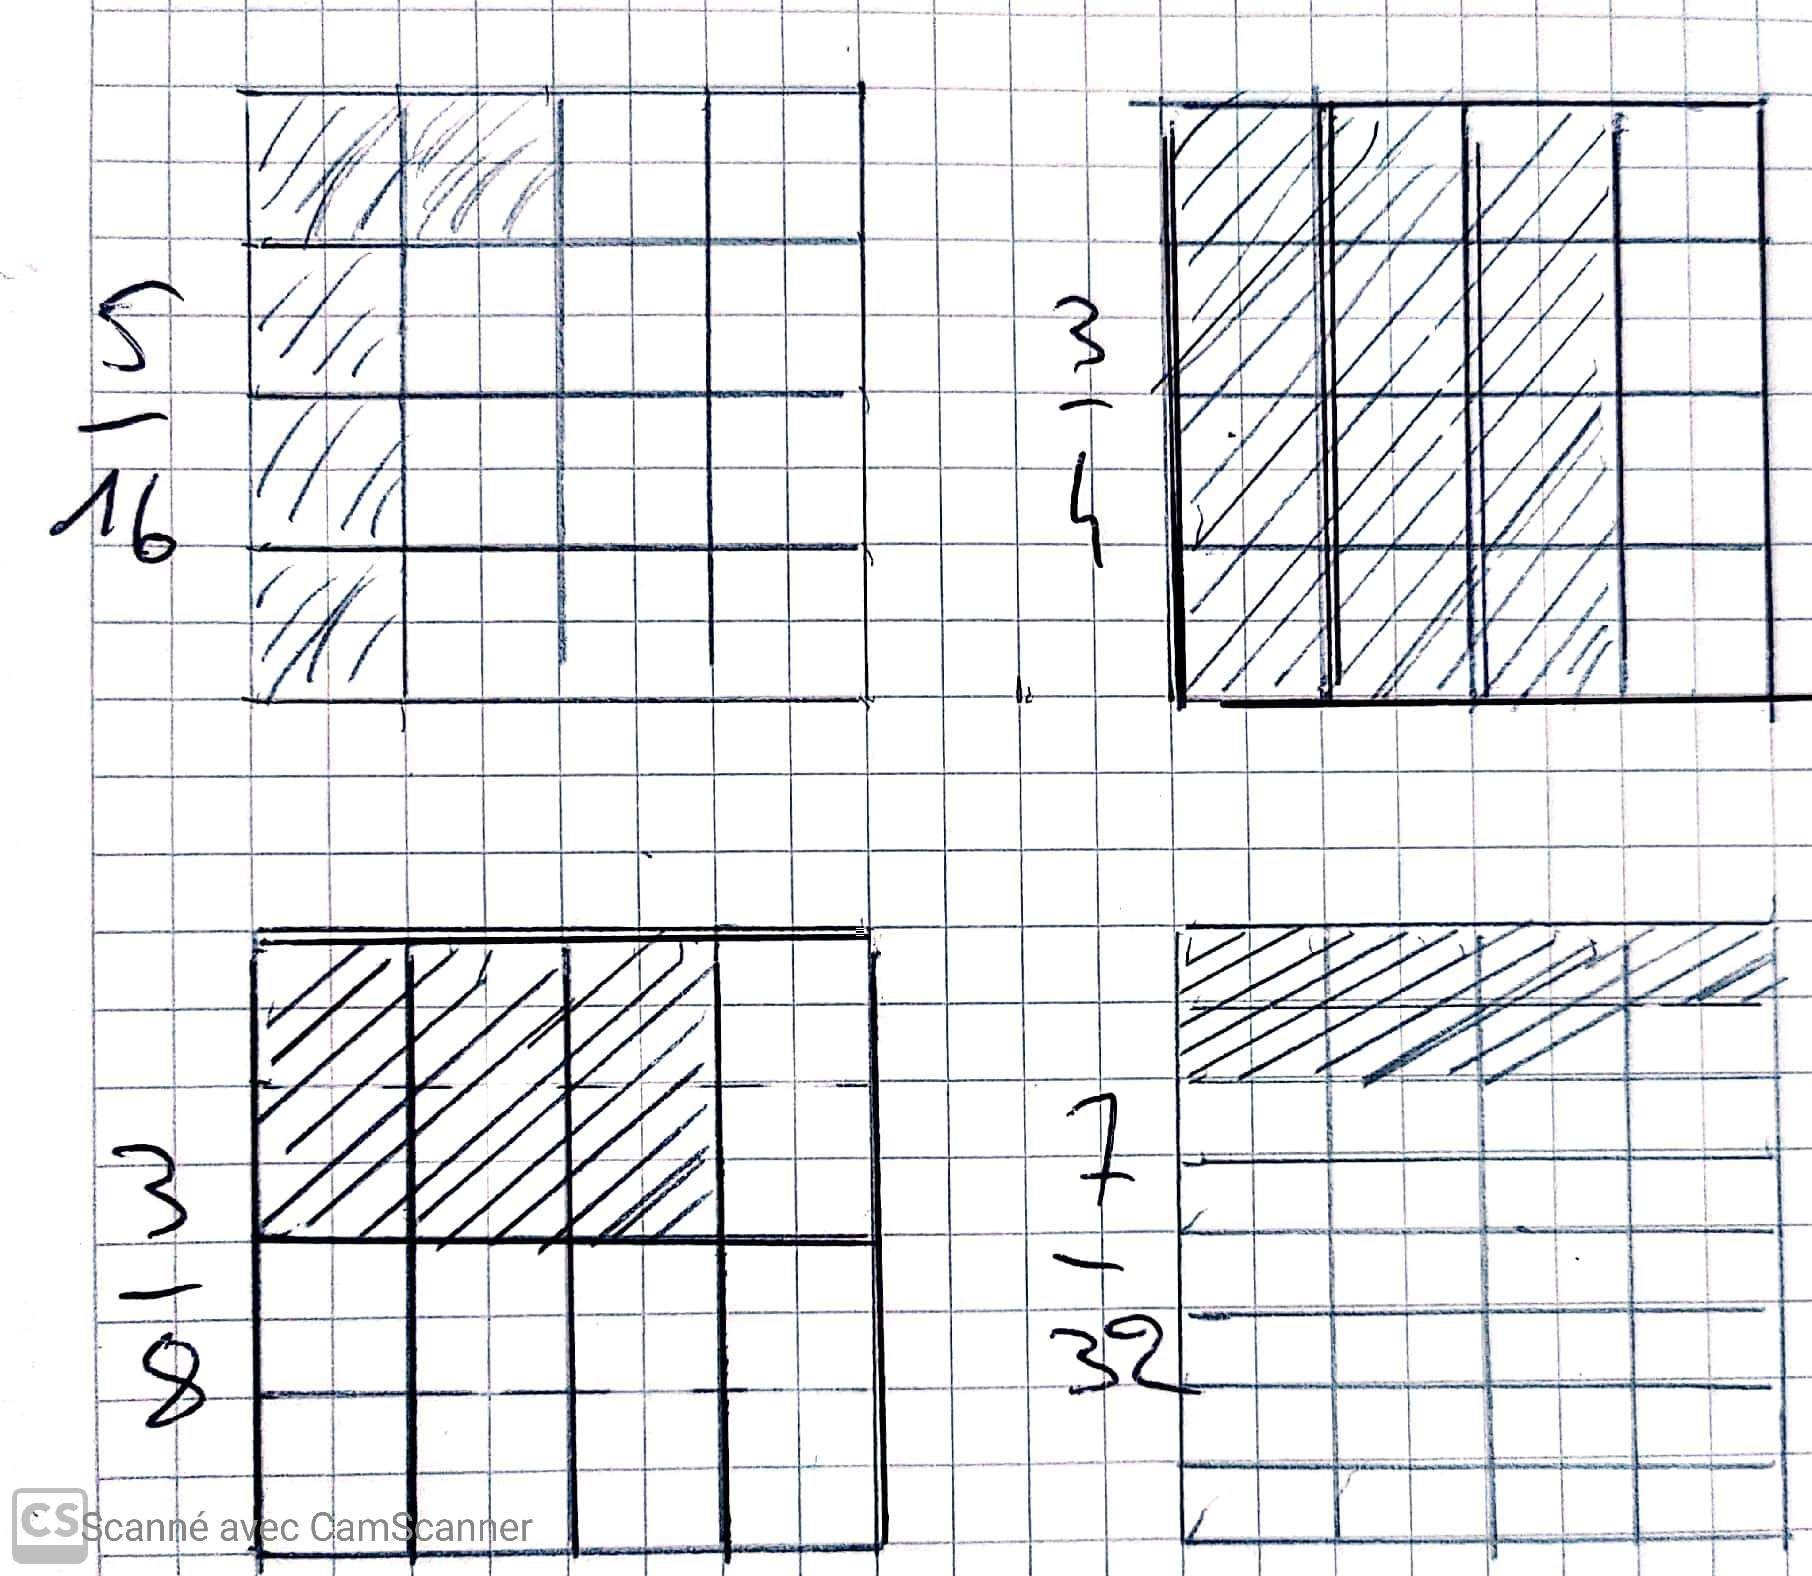
\includegraphics[scale=0.18]{img/ex3}
\end{center}
%\begin{tikzpicture}
%\draw (0,0) rectangle (1,1) ;
%\draw (1,0) rectangle (2,1) ;
%\draw (2,0) rectangle (3,1) ;
%\draw (3,0) rectangle (4,1) ;
%
%\draw (0,1) rectangle (1,2) ;
%\draw (1,1) rectangle (2,2) ;
%\draw (2,1) rectangle (3,2) ;
%\draw (3,1) rectangle (4,2) ;
%
%\draw (0,2) rectangle (1,3) ;
%\draw (1,2) rectangle (2,3) ;
%\draw (2,2) rectangle (3,3) ;
%\draw (3,2) rectangle (4,3) ;
%
%
%\draw (0,3) rectangle (1,4) ;
%\draw (1,3) rectangle (2,4) ;
%\draw (2,3) rectangle (3,4) ;
%\draw (3,3) rectangle (4,4) ;
%
%\end{tikzpicture}


\section{Exercice 5 page 75}

Le digramme est partagé en 12 parts, 2 sont oranges, 3 sont bleues et 7 sont vertes. 
Donc Laurent a reçu $\dfrac{7}{12}$ des voix, Marion $\dfrac{3}{12}$ et Salim $\dfrac{2}{12}$.

\section{Exercice 6 page 75}

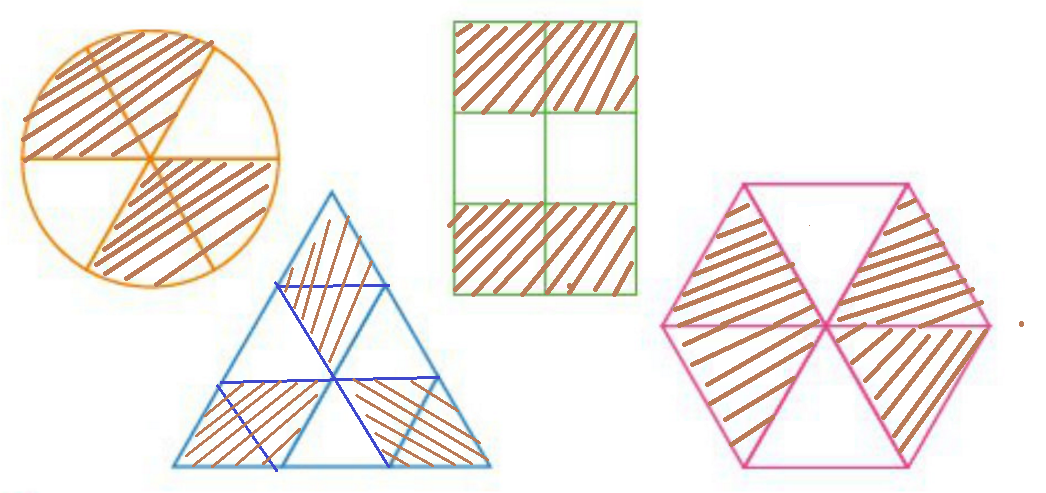
\includegraphics[scale=0.5]{img/ex6}


\section{Exercice 4 page 74}

\begin{enumerate}
	\item Dans cette question, l'unité est partagée en 5 parties,  donc :
	
	\begin{multicols}{2}
		\begin{itemize}
			\item L'abscisse de A est $\dfrac{1}{5}$
			\item L'abscisse de B est $\dfrac{7}{5}$
			\item L'abscisse de C est $\dfrac{9}{5}$
			\item L'abscisse de D est $\dfrac{12}{5}$
			
		\end{itemize}
	\end{multicols}
	

	\item Dans cette question, l'unité est partagée en 6 parties,  donc :
	
	\begin{multicols}{2}
			\begin{itemize}
				\item L'abscisse de A est $\dfrac{5}{6}$
				\item L'abscisse de B est $\dfrac{9}{6}$
				\item L'abscisse de C est $\dfrac{10}{6}$
				\item L'abscisse de D est $\dfrac{14}{6}$
				
			\end{itemize}
	\end{multicols}
	
\end{enumerate}

\section{Exercice 8 page 75}

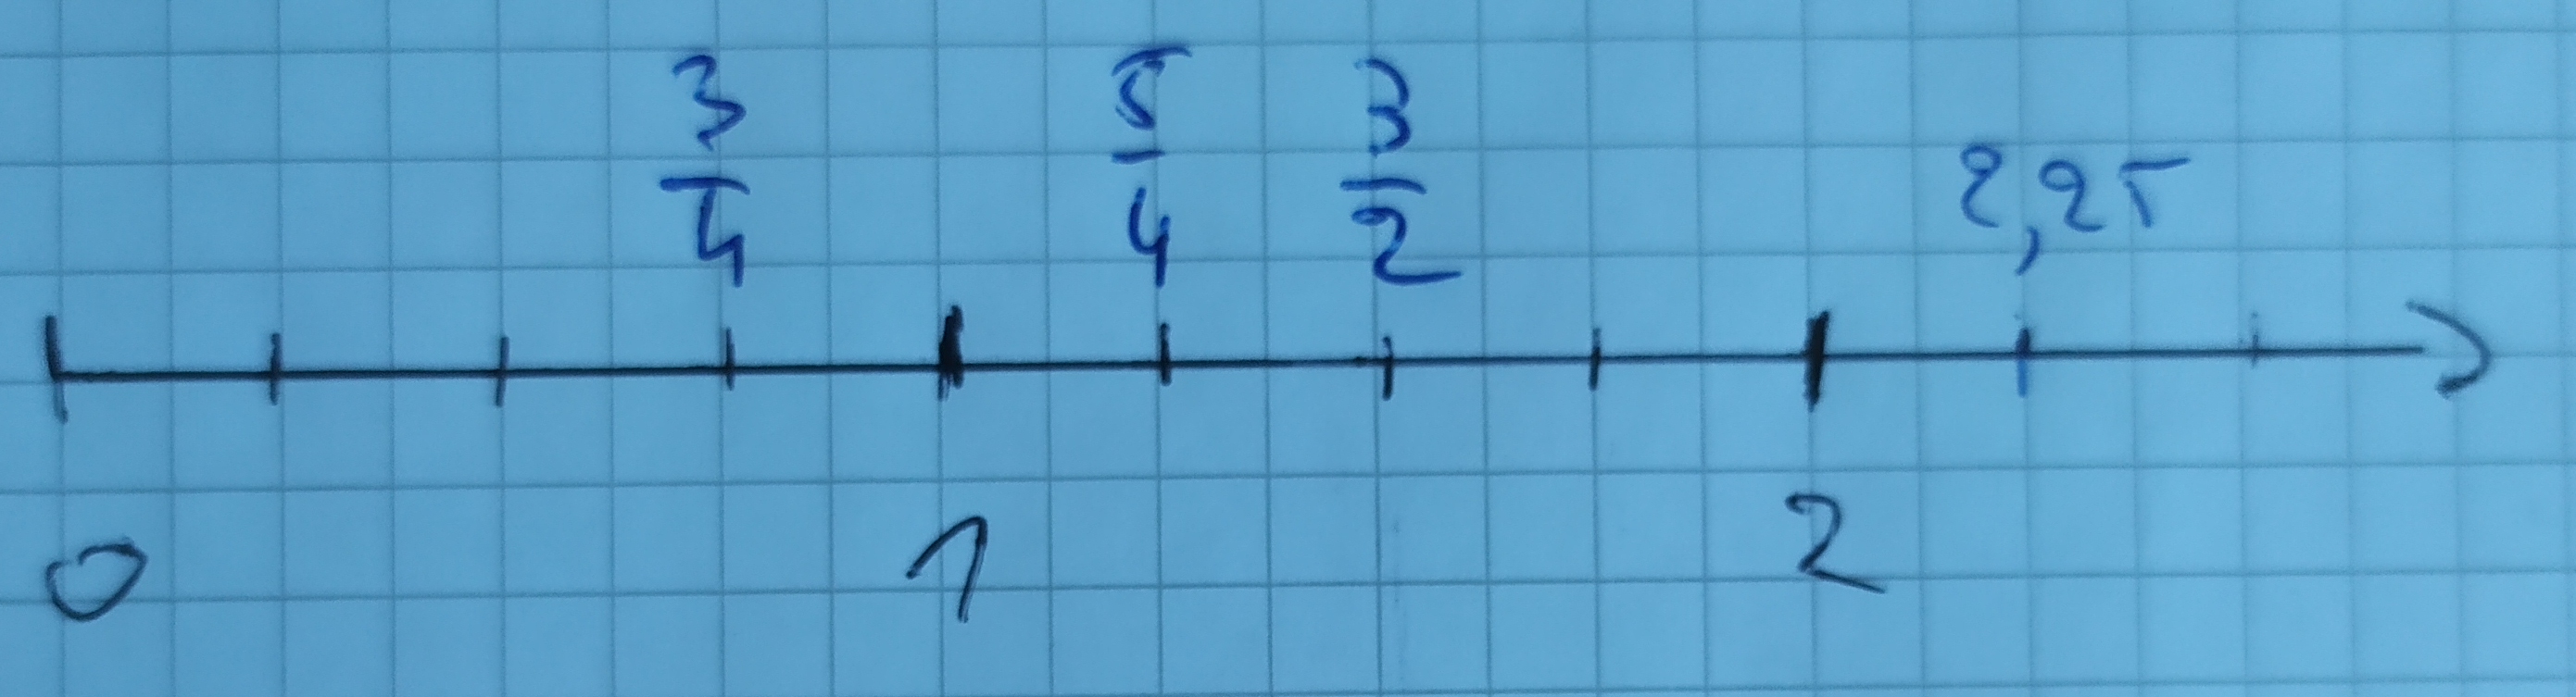
\includegraphics[scale=0.17]{img/ex8}

\vspace*{0.25cm}

Le nombre le plus grand est $\num{2.25}$, le plus petit est $\dfrac{3}{4}$.


\section{Exercice 9 page 75}

\includegraphics[scale=0.2]{img/ex9}

On a donc :

\begin{multicols}{3}
	\begin{itemize}
		\item $\dfrac{3}{5} <  \dfrac{4}{6}$
		\item $\dfrac{13}{6} <  \dfrac{9}{4}$
		\item $\dfrac{5}{4} <  \dfrac{7}{5}$
	\end{itemize}
\end{multicols}
\section{Exercice 10 page 75}

\begin{enumerate}
	\item \ \\
	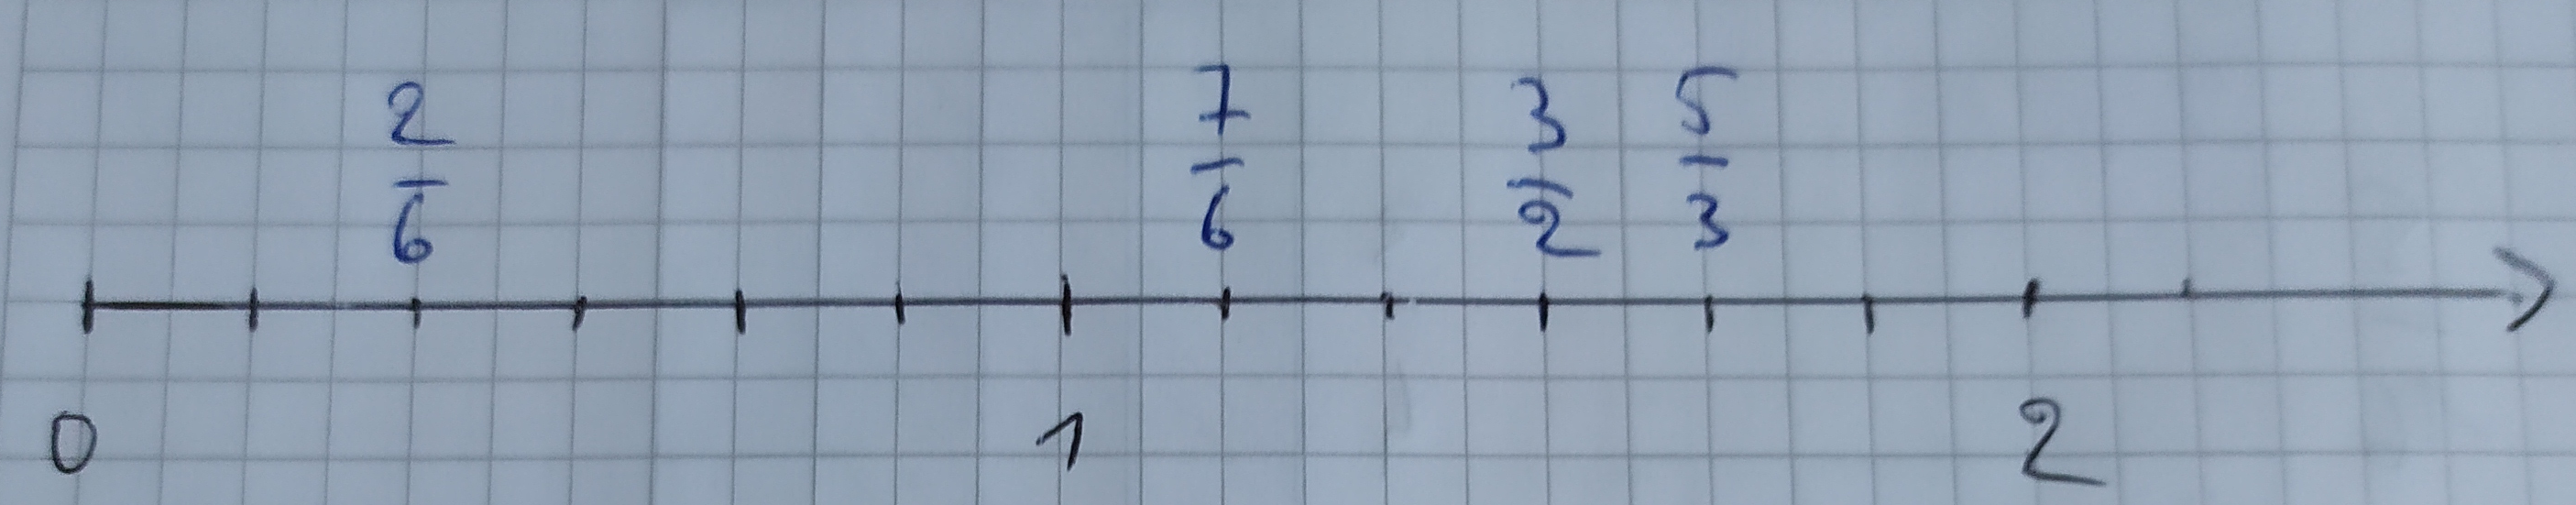
\includegraphics[scale=0.2]{img/ex10}
	
	\item Donc $\dfrac{2}{6} < \dfrac{7}{6} < \dfrac{3}{2} < \dfrac{5}{3}$ .
\end{enumerate}


\end{document}
